\def\sniper{
    Xuất phát từ những vấn đề tồn đọng của phương pháp SNIP, nhóm tác giả \cite{singh2018sniper} đã đề xuất phương pháp chuẩn bị dữ liệu Scale Normalization for Image Pyramids with Efficient Resampling (gọi tắt là SNIPER).
    Phương pháp chuẩn bị dữ liệu SNIPER hướng đến việc giảm thiểu đến tối đa khối lượng tính toán dư thừa từ đó tăng tốc được quá trình train mô hình.
    Nhóm tác giả đã thành công trong việc duy trì được kết quả mà SNIP đạt được trong khi SNIPER chỉ cần xử lý số lượng pixel ảnh bằng một phần ba số lượng mà SNIP phải xử lý.
    Điều này giúp việc train bằng phương pháp SNIPER tiết kiệm bộ nhớ hơn và có thể sử dụng được batch size lớn hơn trong quá trình train.
    Mô hình object detection mà nhóm tác giả sử dụng để làm các thí nghiệm với SNIPER là mô hình Faster R-CNN \cite{ren2015faster}.

    \noindent
    \textbf{\textit{Ý tưởng của phương pháp chuẩn bị dữ liệu SNIPER}} \\
    Nhằm tối ưu hoá khối lượng tính toán trong quá trình train, thay vì việc thay đổi kích thước của ảnh và chọn ra những object có kích thước phù hợp trong quá trình train, phương pháp SNIPER cung cấp một cơ chế tiền xử lý dữ liệu.
    Từ bộ dữ liệu gốc ban đầu, các thuật toán của SNIPER xử lý và tạo ra bộ dữ liệu mới với các ảnh trong bộ dữ liệu được gọi là các Chip.

    \noindent
    \textbf{\textit{Định nghĩa Chip và phương pháp sinh ra Chip bằng phương pháp chuẩn bị dữ liệu SNIPER}} \\
    Chip trong SNIPER có thể được hiểu là một phần của bức ảnh và đây cũng là đơn vị dữ liệu sử dụng trong quá trình train mô hình.
    Các bước sinh ra bộ Chip trong thuật toán SNIPER như sau: \\
    - \textit{Bước 1}: Nhóm tác giả định nghĩa một danh sách các kích thước ảnh {${s}_{1}$, ${s}_{2}$, ..., ${s}_{i}$, ..., ${s}_{n}$}. \\
    - \textit{Bước 2}: SNIPER thay đổi kích thước của từng ảnh gốc ban đầu về từng kích ${s}_{i}$ trong danh sách trên.
    Ta thu được một bộ dữ liệu ảnh mới, trong đó, mỗi ảnh trong bộ dữ liệu ảnh ban đầu tương ứng với n ảnh với các kích thước khác nhau trong bộ dữ liệu ảnh mới. \\
    - \textit{Bước 3}: Trên mỗi ảnh trong bộ dữ liệu ảnh mới, SNIPER đặt các ô vuông có kích thước \textit{KxK} sao cho tâm của các ô vuông này cách đều nhau một khoảng \textit{d} pixel. \\
    - \textit{Bước 4}: SNIPER cắt ảnh theo các ô vuông đã đặt từ bước 3 để tạo thành các Chip. Danh sách các Chip này sẽ được lựa chọn và xử lý ở các thuật toán tiếp theo.

    \noindent
    \textbf{\textit{Phương pháp lựa chọn các positive Chips}} \\
    Từ danh sách các Chip đã được tạo ra bởi thuật toán trên, nhóm tác giả thực hiện thuật toán lựa chọn các positive Chips.
    positive Chip ở đây được hiểu là các Chip chứa các groundtruth bounding box của object mà mô hình cần học.
    Các bước lựa chọn ra positive Chip trong phương pháp SNIPER như sau: \\
    - \textit{Bước 1}: Nhóm tác giả định nghĩa một danh sách các khoảng kích thước bounding box phù hợp tương ứng với mỗi kích thước ảnh {${s}_{1}$, ..., ${s}_{n}$}.
    Cụ thể, với kích thước ảnh ${s}_{i}$, ta định nghĩa khoảng kích thước bounding box phù hợp ${R}^{i} = [{r}_{min}^{i}, {r}_{max}^{i}]$. \\
    - \textit{Bước 2}: SNIPER kiểm tra từng bounding box trong từng Chip trên từng kích thước ảnh.
    Những bounding box có kích thước nằm trong khoảng kích thước phù hợp ${R}^{i}$ được thêm vào danh sách các bounding box hợp lệ ${G}^{i}$. \\
    - \textit{Bước 3}: SNIPER lựa chọn các Chip từ danh sách các Chip ở thuật toán trên sao cho số lượng bounding box hợp lệ và nằm hoàn toàn trong một Chip là nhiều nhất.
    Danh sách các positive Chips trên mỗi ảnh trong cùng một kích thước được gọi là ${C}_{pos}^{i}$.

    \begin{figure}[H]
        \centering
        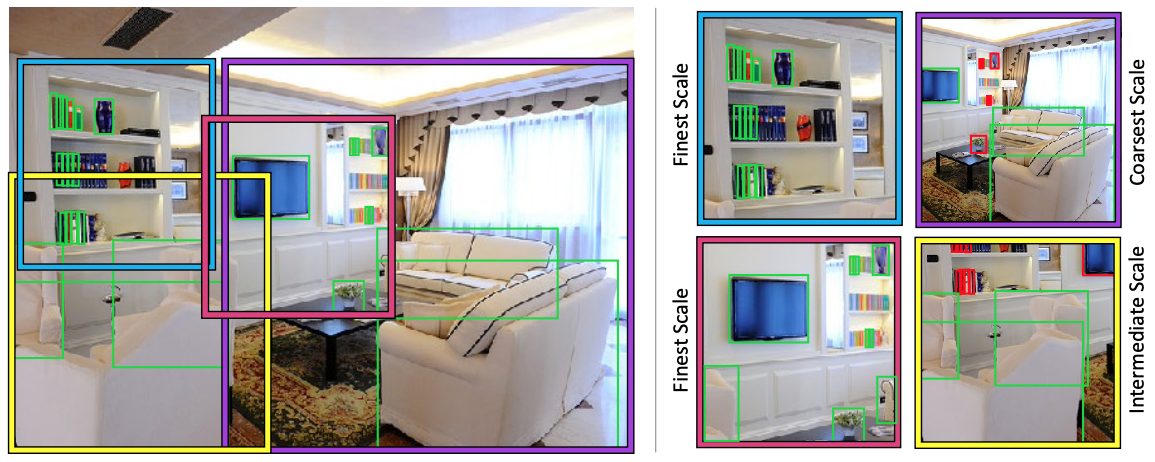
\includegraphics[width=13cm] {images/sniper_pos_chip}
        \caption{Kết quả thuật toán lựa chọn các positive chips (Nguồn: \cite{singh2018sniper})}
        \label{fig:sniper_pos_chip}
    \end{figure}

    \noindent
    Một groundtruth bounding box bất kỳ sẽ luôn có một Chip nào đó chứa nó và có thể xuất hiện ở nhiều hơn một Chip trong cùng một kích thước ảnh hoặc trong nhiều kích thước ảnh khác nhau.
    Các groundtruth bounding box không nằm hoàn toàn trong một chip sẽ bị cắt.
    Phần cắt nếu thoả mãn khoảng kích thước phù hợp sẽ được coi là hợp lệ, phần cắt nếu không thoả mãn khoảng kích thước phù hợp sẽ được coi là vi phạm nhưng vẫn được sử dụng để gán label cho các khu vực được đề xuất bởi mô hình RPN. \\
    Mỗi groundtruth bounding box tìm được kích thước Chip phù hợp để học, và hơn nữa kích thước của mỗi Chip nhỏ hơn rất nhiều so với mỗi kích thước ảnh tương ứng của Chip đó.
    Điều này mang lại sự tiết kiệm trong cả nguồn bộ nhớ lẫn tốc độ tính toán. \\
    Trong hình \ref{fig:sniper_pos_chip}, từ ảnh và các groundtruth bounding box ban đầu (ảnh bên phải), thuật toán của SNIPER đã cắt ra được các Chip (ảnh bên trái), mỗi Chip sẽ tương ứng chứa các groundtruth bounding box hợp lệ (các bounding box màu xanh) và các groundtruth bounding box không hợp lệ (các bounding box màu đỏ).
    Kết quả trên của SNIPER đảm bảo tất cả các groundtruth bounding box đều được train ở một Chip nào đó phù hợp, trong khi kích thước của Chip chỉ bằng 1/10 kích thước của ảnh phù hợp cho groundtruth bounding box.

    \noindent
    \textbf{\textit{Phương pháp lựa chọn các negative Chips}} \\
    Việc xây dựng thuật toán lựa chọn các positive Chips chứa tất cả các groundtruth bounding box đã giúp cải thiện rất nhiều tốc độ train mô hình.
    Nhưng vẫn còn một vấn đề tồn đọng, đó chính là việc thiếu hụt một lượng lớn background (do phần lớn background đã bị loại bỏ trong thuật toán sinh ra các positive Chips).
    Điều này dẫn đến việc mô hình thường xuyên dự đoán background thành các vùng chứa các đối tượng.
    Do đó, nhóm tác giả đề xuất bổ sung thêm các Chip là background không chứa đối tượng, gọi là các negative Chips. \\
    Nhóm tác giả nhận xét rằng có một số phần background trong ảnh rất dễ để phân biệt và sẽ tốn kém chi phí tính toán để xử lý những phần background dễ này.
    Từ nhận xét trên, nhóm tác giả đề xuất việc sử dụng các khu vực được đề xuất từ mô hình Region Proposal Network của Faster R-CNN bởi vì các khu vực này có khả năng khiến cho mô hình nhầm lẫn giữa đối tượng cụ thể nào đó và background.

    \begin{figure}[H]
        \centering
        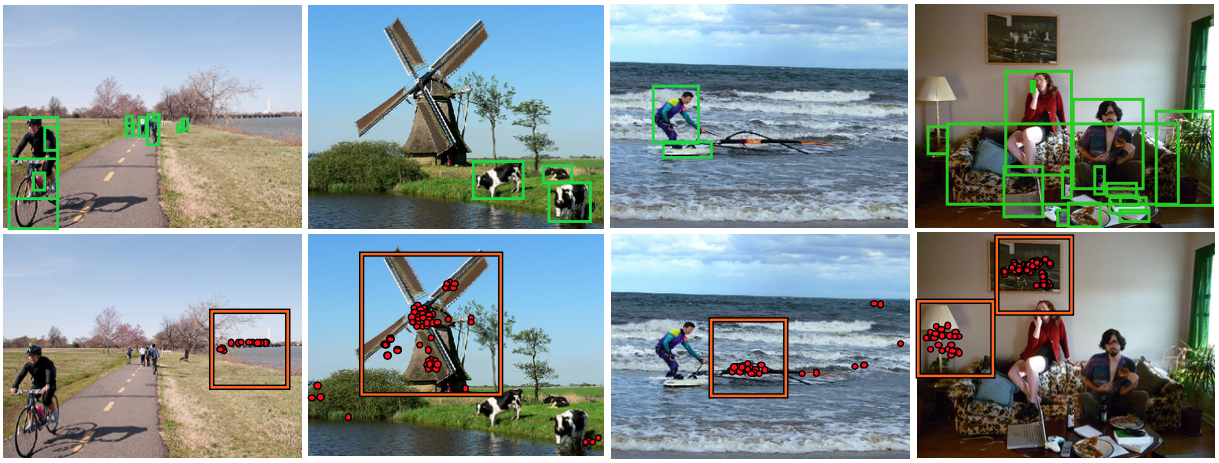
\includegraphics[width=13cm] {images/sniper_neg_chip}
        \caption{Kết quả thuật toán lựa chọn các negative chips (Nguồn: \cite{singh2018sniper})}
        \label{fig:sniper_pos_chip}
    \end{figure}

    \noindent
    Các bước lựa chọn negative Chips trong phương pháp SNIPER như sau: \\
    \textit{Bước 1}: SNIPER train RPN của mô hình Faster R-CNN một vài epoch với chỉ các positive Chips. \\
    \textit{Bước 2}: SNIPER sử dụng mô hình RPN đã được train từ bước 1 để thực hiện dự đoán các khu vực đề xuất trong bộ dữ liệu train (ảnh trong bộ dữ liệu train lúc này cũng được thay đổi kích thước {${s}_{1}$, ..., ${s}_{n}$} như thuật toán lựa chọn positive Chips).
    Các khu vực không được RPN dự đoán sẽ được coi là những khu vực background dễ học và loại các khu vực đó ra khỏi quá tình lựa chọn negative Chips. \\
    \textit{Bước 3}: Từ những khu vực mà RPN dự đoán, đầu tiên, SNIPER loại các khu vực nằm trong danh sách positive Chips.
    Các Chips sẽ được lựa chọn nếu chứa nhiều hơn M khu vực được đề xuất tạo thành danh sách các negative Chips ${C}_{neg}^{i}$. \\
    \textit{Bước 4}: Danh sách các negative Chips được kết hợp cùng với danh sách các positive Chips để tiếp tục train mô hình Faster R-CNN.

    \noindent
    \textbf{\textit{Kết quả của mô hình SNIPER}} \\
    Theo thống kê của nhóm tác giả trên bộ dữ liệu COCO, bằng các phương pháp sinh và lựa chọn Chips, số lượng pixel mà SNIPER xử lý trong quá trình train chỉ hơn khoảng 30\% so với số lượng pixel cần xử lý khi train với chỉ duy nhất một kích thước của ảnh.
    So sánh với việc train với dữ liệu ảnh với 3 kích thước khác nhau cho mỗi ảnh, việc sử dụng các Chips có kích thước giống nhau giúp SNIPER tối ưu về batch size hơn khi train mô hình.
    So sánh với chiến lược của SNIP, SNIPER đạt được độ chính xác tương đương trong khi giảm được 3 lần số pixel cần phải train trên bộ dữ liệu COCO.

    \noindent
    \textbf{\textit{Vấn đề tồn đọng của mô hình SNIPER}} \\
    SNIPER đã phần nào đó cải thiện một cách đáng kể vấn đề về thời gian train của SNIP.
    Tuy nhiên, trong quá trình dự đoán, SNIPER vẫn cần phải sử dụng phương pháp Image Pyramids để đạt được độ chính xác cao.
    Đối với những bộ dữ liệu ảnh có kích thước lớn thì tốc độ dự đoán của SNIPER vẫn rất chậm và đây là vấn đề tồn đọng thúc đẩy các nghiên cứu giải quyết triệt để.
}